% 例 2：正方形 ABCD 内一点 P，把 △ABP 绕 A 顺时针 90° 得 △ADP'
\documentclass[tikz,border=4pt]{standalone}
\usepackage{ctex}
\usepackage{amsmath}
\usetikzlibrary{calc, arrows.meta}
\begin{document}
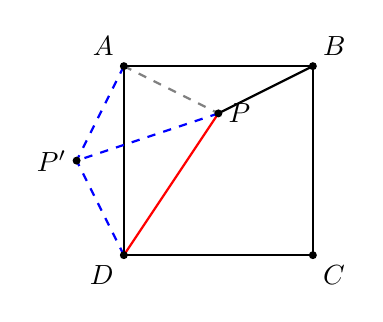
\begin{tikzpicture}[scale=1.2, thick]
  \coordinate (A) at (0,2);
  \coordinate (B) at (2,2);
  \coordinate (C) at (2,0);
  \coordinate (D) at (0,0);
  \coordinate (P) at (1.0, 1.5);
  % 绕 A 顺时针 90°：B(2,2)->D(0,0)? 取 A 为旋转中心，向量 (B-A)=(2,0) 顺时针90°→(0,-2)，A+(0,-2)=(0,0)=D ✓
  % P-A=(1,-0.5) 顺时针90°→(-0.5,-1)，加 A → (-0.5,1) 这是 P'
  \coordinate (Pp) at (-0.5, 1);

  \draw (A) -- (B) -- (C) -- (D) -- cycle;
  \draw[gray, dashed] (A) -- (P);
  \draw (B) -- (P);
  \draw[red] (P) -- (D); % PD 目标
  \draw[blue, dashed] (A) -- (Pp);
  \draw[blue, dashed] (D) -- (Pp);
  \draw[blue, dashed] (P) -- (Pp);

  \fill (A) circle (1.2pt); \fill (B) circle (1.2pt);
  \fill (C) circle (1.2pt); \fill (D) circle (1.2pt);
  \fill (P) circle (1.2pt); \fill (Pp) circle (1.2pt);
  \node[above left] at (A) {$A$};
  \node[above right] at (B) {$B$};
  \node[below right] at (C) {$C$};
  \node[below left] at (D) {$D$};
  \node[right] at (P) {$P$};
  \node[left] at (Pp) {$P'$};
\end{tikzpicture}
\end{document}
